\section{回归分析}
    \begin{enumerate}
        \item
        \code
\begin{lstlisting}
x <- read.table("ex4_1-data.txt", header=TRUE)
lm.1 <- lm(Y~X1+X2, data=x)
summary(lm.1)
R = sqrt(summary(lm(Y~X1+X2, data=x))$r.sq); R
\end{lstlisting}
        \out
\begin{lstlisting}
> summary(lm.1)

Call:
lm(formula = Y ~ X1 + X2, data = x)

Residuals:
    Min      1Q  Median      3Q     Max 
-3.9340 -0.8672  0.5711  0.7114  4.4507 

Coefficients:
             Estimate Std. Error t value Pr(>|t|)    
(Intercept) -61.47289   17.60192  -3.492  0.00580 ** 
X1            2.12039    0.18148  11.684 3.75e-07 ***
X2            0.39431    0.08631   4.569  0.00103 ** 
---
Signif. codes:  0 ‘***’ 0.001 ‘**’ 0.01 ‘*’ 0.05 ‘.’ 0.1 ‘ ’ 1

Residual standard error: 2.968 on 10 degrees of freedom
Multiple R-squared:  0.9417,	Adjusted R-squared:  0.9301 
F-statistic: 80.83 on 2 and 10 DF,  p-value: 6.709e-07

> R
[1] 0.9704358
\end{lstlisting}
        \summary\\
        根据输出,可以得到
        \begin{enumerate}[label=(\arabic*)]
            \item $Y$关于$X_1,X_2$的二元线性回归方程为
            \[Y=-61.47289+2.12039X_1+0.39431X_2.\]
            \item 自变量$X_1$的系数$p$值为$3.75\times 10^{-7}<0.05$,认为$X_1$在0.05的显著性水平下是显著的;\\自变量$X_2$的系数$p$值为$0.00103<0.05$,认为$X_2$在0.05的显著性水平下是显著的;
            \item 复相关系数为0.9704358。
        \end{enumerate}
        \item
        \code
\begin{lstlisting}
x <- read.table("ex4_2-data.txt", header=TRUE)
# (1)
lm.1 <- lm(Y~X1+X2, data=x)
coefficients(lm.1)
# (2)
attach(x)
# 散点图
plot(Y~X1)
abline(lm(Y~X1))
plot(Y~X2)
abline(lm(Y~X2))
# 残差图
resid <- residuals(lm.1)
y.pre <- predict(lm.1)
plot(y.pre, resid)
# 残差QQ图
plot(lm.1,2)
\end{lstlisting}
        \out
\begin{lstlisting}
> coefficients(lm.1)
(Intercept)          X1          X2 
 -4.9513762   1.5465083  -0.9539819
\end{lstlisting}
        \begin{figure}[H]
            \centering
            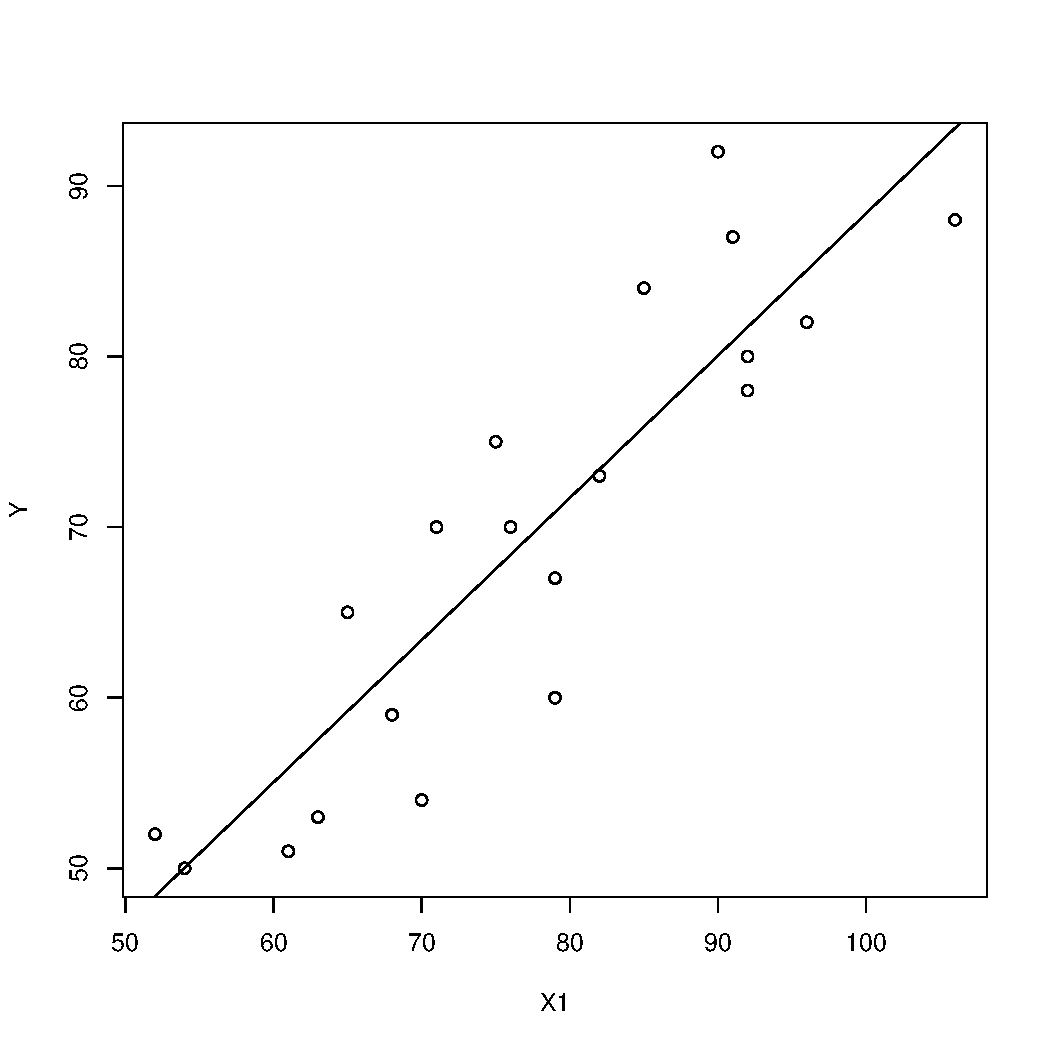
\includegraphics[scale=0.6]{4.2散点图Y-X1.pdf}
            \caption{题2中$Y$关于$X_1$的散点图}
        \end{figure}
        \begin{figure}[H]
            \centering
            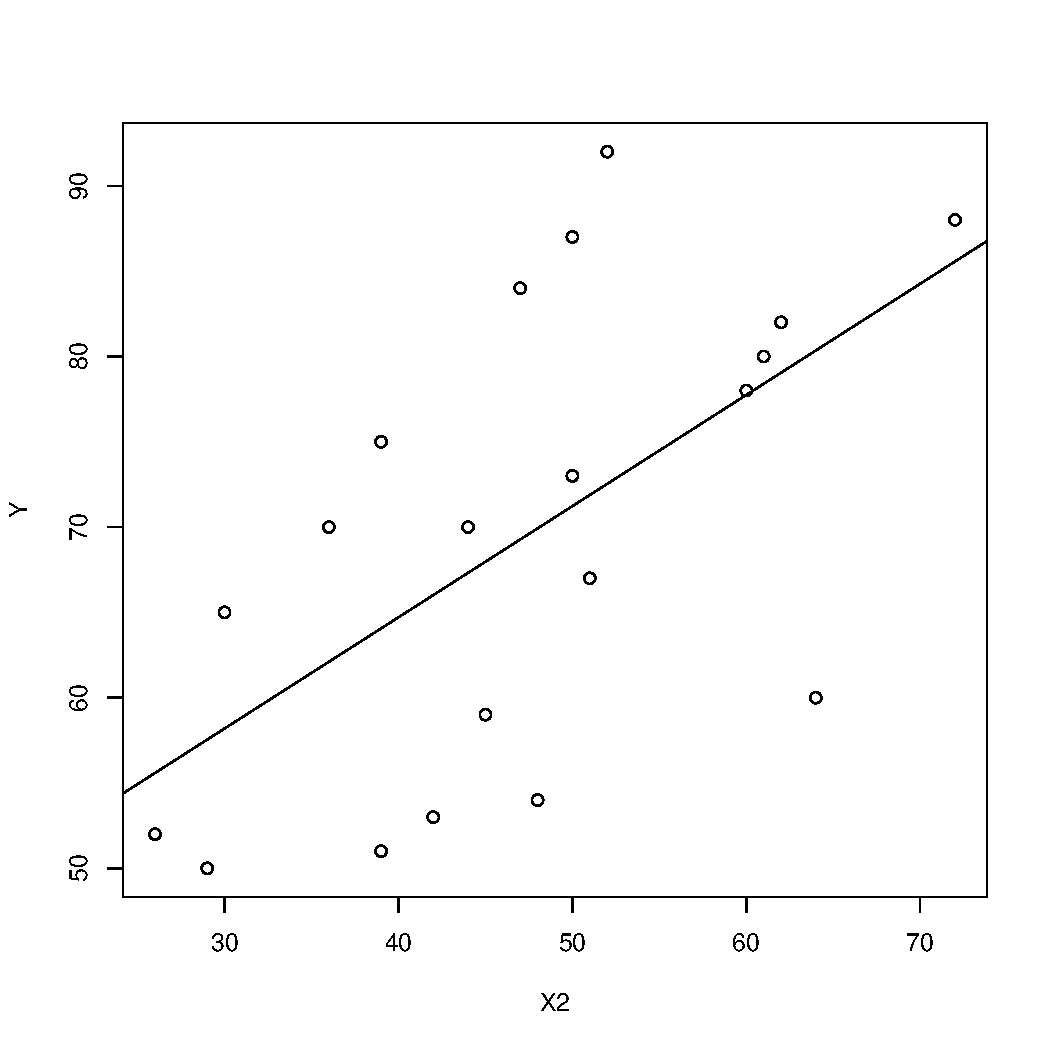
\includegraphics[scale=0.6]{4.2散点图Y-X2.pdf}
            \caption{题2中$Y$关于$X_2$的散点图}
        \end{figure}
        \begin{figure}[H]
            \centering
            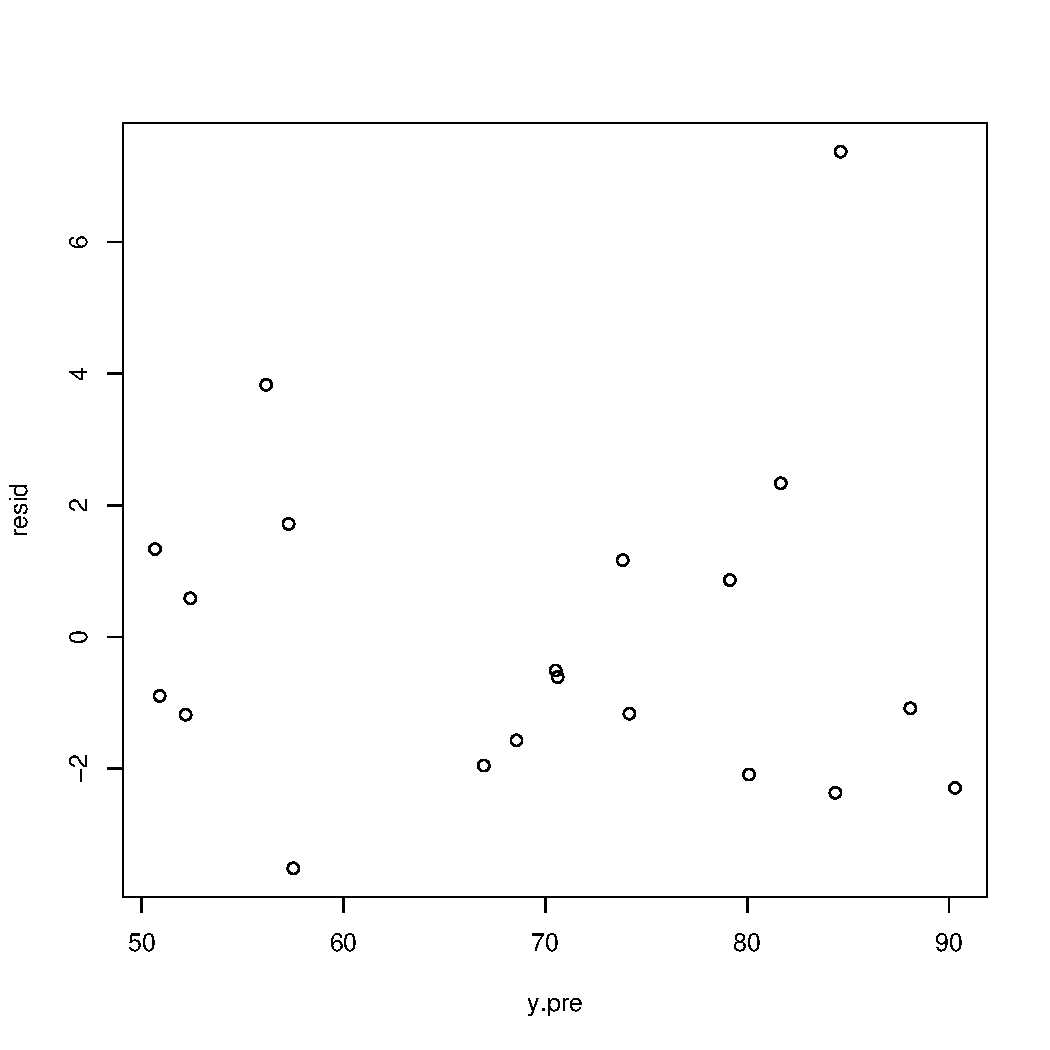
\includegraphics[scale=0.6]{4.2残差图.pdf}
            \caption{题2中的残差图}
        \end{figure}
        \begin{figure}[H]
            \centering
            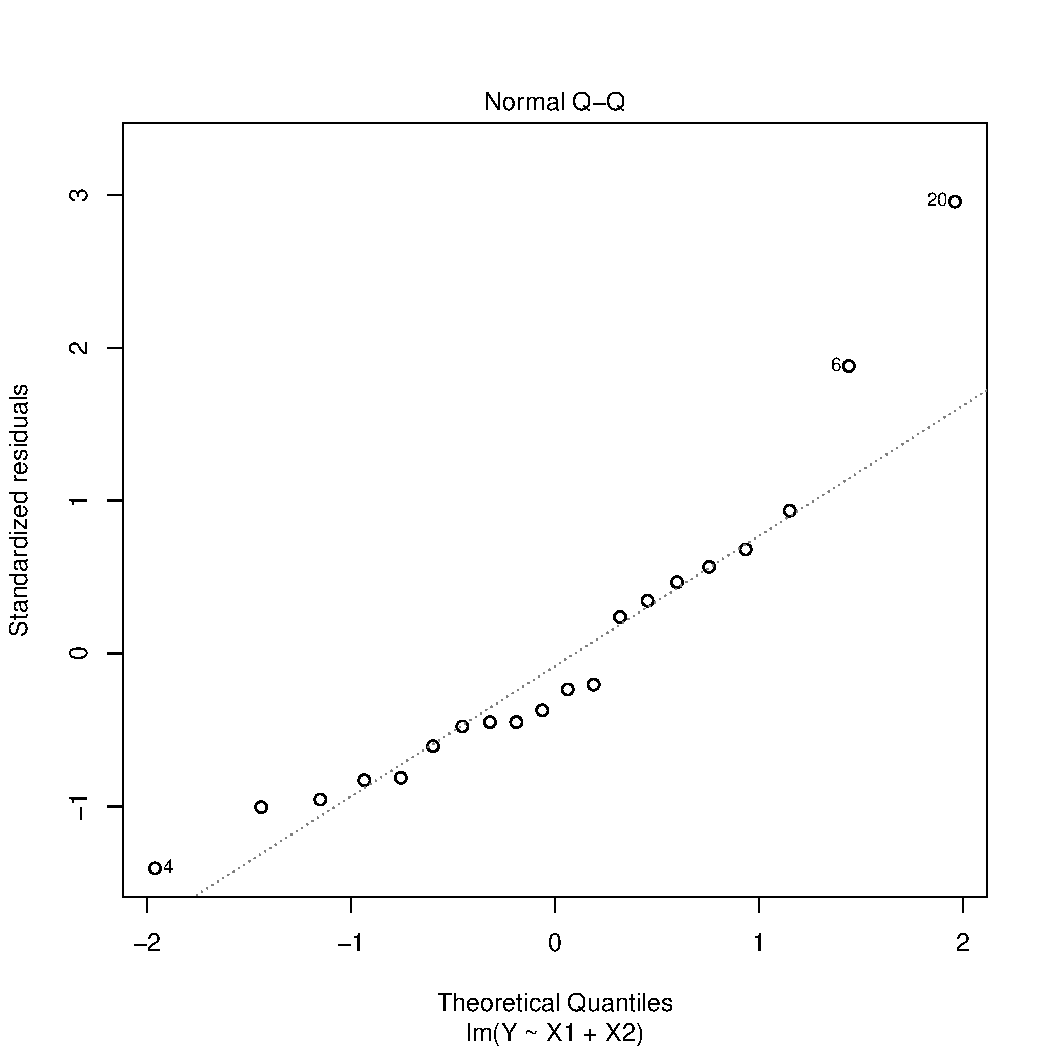
\includegraphics[scale=0.6]{4.2残差QQ图.pdf}
            \caption{题2中的残差QQ图}
        \end{figure}
        \summary\\
        根据输出,可以得到
        \begin{enumerate}[label=(\arabic*)]
            \item $Y$关于$X_1,X_2$的二元线性回归方程为
            \[Y=-4.9513762+1.5465083X_1-0.9539819X_2.\]
            \item 通过两张散点图和残差图,可以认为残差随时间变换呈线性变化,因此回归函数中应包含时间的线性项;\\
            通过残差QQ图,可以认为残差所属总体为$N(0,1)$,因此总体分布是正态分布。
        \end{enumerate}
        \item
        \code
\begin{lstlisting}
x <- read.table("ex4_3-data.txt", header=TRUE)
source("step.regression.R")
step.regression(x, x[[6]], c(2,3,4,5), 0.05, 0.05)
attach(x)
lm.1 <- lm(Y2~Y1+X3+X2, data=x)
summary(lm.1)
\end{lstlisting}
        \out
\begin{lstlisting}
> step.regression(x, x[[6]], c(2,3,4,5), 0.05, 0.05)
  Varible Enter.Exclude    F.value     P.value
1      Y1         Enter 173.500426 0.000000000
2      X3         Enter   8.307257 0.005765805
3      X2         Enter  11.918944 0.001139657

> summary(lm.1)

Call:
lm(formula = Y2 ~ Y1 + X3 + X2, data = x)

Residuals:
     Min       1Q   Median       3Q      Max 
-0.28869 -0.04378  0.00621  0.04249  0.56721 

Coefficients:
             Estimate Std. Error t value Pr(>|t|)    
(Intercept) 1.3542790  0.1177948  11.497 1.20e-15 ***
Y1          0.0010070  0.0001892   5.322 2.43e-06 ***
X3          0.0048378  0.0010773   4.491 4.20e-05 ***
X2          0.0045750  0.0013252   3.452  0.00114 ** 
---
Signif. codes:  0 ‘***’ 0.001 ‘**’ 0.01 ‘*’ 0.05 ‘.’ 0.1 ‘ ’ 1

Residual standard error: 0.1169 on 50 degrees of freedom
Multiple R-squared:  0.8399,	Adjusted R-squared:  0.8303 
F-statistic: 87.42 on 3 and 50 DF,  p-value: < 2.2e-16
\end{lstlisting}
        \summary\\
        根据输出,所得最优回归方程为\[Y_2 = 1.3542790+0.0010070Y_1+0.0048378X_3+0.0045750X_2.\]
        \item
        \code
\begin{lstlisting}
x <- read.table("ex4_4-data.txt", header=TRUE)
log.lm <- glm(Y~X1+X2+X3, family=binomial, data=x)
summary(log.lm)
\end{lstlisting}
        \out
\begin{lstlisting}
> summary(log.lm)

Call:
glm(formula = Y ~ X1 + X2 + X3, family = binomial, data = x)

Deviance Residuals: 
    Min       1Q   Median       3Q      Max  
-1.4903  -0.8790  -0.7097   0.9873   1.7984  

Coefficients:
            Estimate Std. Error z value Pr(>|z|)  
(Intercept) -0.03785    0.92265  -0.041   0.9673  
X1          -1.70448    0.71784  -2.374   0.0176 *
X2           0.01118    0.01771   0.631   0.5280  
X3           0.30887    0.70744   0.437   0.6624  
---
Signif. codes:  0 ‘***’ 0.001 ‘**’ 0.01 ‘*’ 0.05 ‘.’ 0.1 ‘ ’ 1

(Dispersion parameter for binomial family taken to be 1)

    Null deviance: 61.29  on 44  degrees of freedom
Residual deviance: 54.70  on 41  degrees of freedom
AIC: 62.7

Number of Fisher Scoring iterations: 4
\end{lstlisting}
        \summary\\
        根据输出,所得关系为
        \[P\{Y=1\}=\frac{\exp(-0.03785-1.70448X_1+0.01118X_2+0.30887X_3)}{1+\exp(-0.03785-1.70448X_1+0.01118X_2+0.30887X_3)}.\]
    \end{enumerate}
\clearpage